\chapter{Gradient methods}


\section{Minimum of a function}

Let $f: \mathbb{R}^N \rightarrow \mathbb{R}$ be continuous and differentiable in $\mathbb{R}^N$.
\begin{descriptionlist}
    \item[Stationary point] \marginnote{Stationary point}
        $\vec{x}^*$ is a stationary point of $f$ iff: 
        \[ \nabla f(\vec{x}^*) = \nullvec \]

    \item[Local minimum] \marginnote{Local minimum}
        $\vec{x}^* \in \mathbb{R}^N$ is a local minimum of $f$ iff:
        \[ f(\vec{x}^*) \leq f(\vec{x}) \text{ } \forall \vec{x} \in \mathbb{R}^N: \Vert \vec{x} - \vec{x}^* \Vert < \varepsilon \]
        
    \item[Strict local minimum] \marginnote{Strict local minimum}
        $\vec{x}^* \in \mathbb{R}^N$ is a strict local minimum of $f$ iff:
        \[ f(\vec{x}^*) < f(\vec{x}) \text{ } \forall \vec{x} \in \mathbb{R}^N: \Vert \vec{x} - \vec{x}^* \Vert < \varepsilon \]

    \item[Global minimum] \marginnote{Global minimum}
        $\vec{x}^* \in \mathbb{R}^N$ is a global minimum of $f$ iff:
        \[ f(\vec{x}^*) \leq f(\vec{x}) \text{ } \forall \vec{x} \in \mathbb{R}^N \]
        
    \item[Strict global minimum] \marginnote{Strict global minimum}
        $\vec{x}^* \in \mathbb{R}^N$ is a strict global minimum of $f$ iff:
        \[ f(\vec{x}^*) < f(\vec{x}) \text{ } \forall \vec{x} \in \mathbb{R}^N \]
\end{descriptionlist}


\subsection{Optimality conditions}

\begin{description}
    \item[First order condition] \marginnote{First order condition}
        Let $f: \mathbb{R}^N \rightarrow \mathbb{R}$ be continuous and differentiable in $\mathbb{R}^N$.
        \[ \text{If } \vec{x}^* \text{ local minimum of } f \Rightarrow \nabla f(\vec{x}^*) = \nullvec \]

    \item[Second order condition] \marginnote{Second order condition}
        Let $f: \mathbb{R}^N \rightarrow \mathbb{R}$ be continuous and twice differentiable.
        \[ 
            \text{If } \nabla f(\vec{x}^*) = \nullvec \text{ and } \nabla^2 f(\vec{x}^*) \text{ positive definite} \Rightarrow 
            \vec{x}^* \text{ strict local minimum of } f 
        \]
\end{description}

As the second order condition requires to compute the Hessian matrix, which is expensive, in practice only the first order condition is checked.



\section{Descent methods}

\marginnote{Descent methods}
Descent methods are iterative methods that have the property:
\[ f(\vec{x}_k) < f(\vec{x}_{k+1}) \]

The iteration is defined as:
\[ \vec{x}_k = \vec{x}_{k-1} + \alpha_{k-1}\vec{p}_{k-1} \]
where $\vec{p}_{k-1} \in \mathbb{R}^N$ is the search direction and \marginnote{Search direction\\Step length}
$\alpha_{k-1} \in \mathbb{R}$ is the step length.

Note: descent methods usually converge to a local minimum.

\begin{figure}
    \centering
    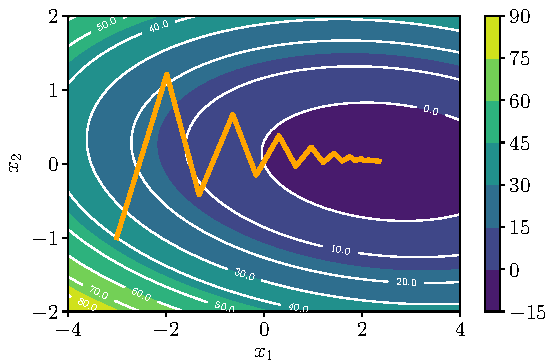
\includegraphics[width=0.5\linewidth]{img/_gradient_contour.pdf}
    \caption{Descent method steps in $\mathbb{R}^2$ (i.e. moving across contour lines)}
\end{figure}


\subsection{Choice of the search direction}

\begin{description}
    \item[Descent direction] \marginnote{Descent direction}
        $\vec{p} \in \mathbb{R}^N$ is a descent direction of $f$ in $\vec{x}$ if:
        \[ \exists \bar{\alpha} > 0, \forall \alpha \in [0, \bar{\alpha}]: f(\vec{x} + \alpha \vec{p}) < f(\vec{x}) \]
\end{description}

\begin{theorem}
    Let $\vec{p} \in \mathbb{R}^N$, $\vec{p} \neq \nullvec$.
    \[ \text{If } \vec{p}^T \nabla f(\vec{x}) < 0 \Rightarrow \vec{p} \text{ descent direction of } f \text{ in } x \]
\end{theorem}

\begin{theorem}
    For all $\vec{x}$, $\vec{p} = -\nabla f(\vec{x})$ is a descent direction of $f$ in $x$.
\end{theorem}
\begin{proof}
    \[
        \begin{split}
            \vec{p}^T \nabla f(\vec{x}) < 0 &\iff -(\nabla f(\vec{x}))^T \nabla f(\vec{x}) < 0 \\
                &\iff - \Vert \nabla f(\vec{x}) \Vert_2^2 < 0
        \end{split}
    \]
    This holds as the norm is always positive.
\end{proof}

\begin{description}
    \item[Gradient-like methods] \marginnote{Gradient-like methods}
        Gradient-like methods are descent methods that use $-\nabla f$ as step.
\end{description}


\subsection{Choice of the step length}
\begin{description}
    \item[Constant] 
        In machine learning, it is common to set a constant value for the step (learning rate), 
        but it can be proved that this does not guarantee convergence.
    
    \item[Backtracking procedure] \marginnote{Backtracking procedure}
        $\alpha_k$ is chose such that it respects the Wolfe condition\footnote{\url{https://en.wikipedia.org/wiki/Wolfe_conditions}}:
        \begin{lstlisting}[mathescape=true, belowskip = -0.8\baselineskip]
            def backtracking($\tau$, $c_1$):
                $\alpha_k$ = 1 # Initial guess
                while $f(x_k - \alpha_k \nabla f(\vec{x}_k))$ > $f(\vec{x}_k)$ + $c_1 \alpha_k \nabla f(\vec{x}_k)^T \nabla f(\vec{x}_k)$:
                    $\alpha_k$ = $\alpha_k$ / $\tau$
                return $\alpha_k$
        \end{lstlisting}
        It can be proved that, by using the backtracking procedure, gradient methods converge to a local minimum.
\end{description}


\subsection{Stopping condition}
\marginnote{Stopping condition}
We can stop iterating when $\vec{x}_k \approx \vec{x}^*$, that is, $\nabla f(\vec{x}_k) \approx \nullvec$.
We can verify this by checking the norm of the gradient against a tolerance $\tau$:
\begin{descriptionlist}
    \item[Absolute condition] $\Vert \nabla f(x_k) \Vert_2 < \tau$ 
    \item[Relative condition] $\frac{\Vert \nabla f(x_k) \Vert_2}{\Vert \nabla f(x_0) \Vert_2} < \tau$ 
\end{descriptionlist}

A generic gradient-like method can then be defined as:
\begin{lstlisting}[mathescape=true]
    def gradientMethod($f$, $\vec{x}_0$):
        $k$ = 0
        while stoppingCondition($f$, $\vec{x}_k$, $\vec{x}_0$):
            $p_k$ = $-\nabla f(\vec{x}_k)$
            $\alpha_k$ = backtracking($\dots$)
            $\vec{x}_{k+1}$ = $\vec{x}_k$ + $\alpha_k \vec{p}_k$
            $k$ = $k$ + 1
        return $x_k$
\end{lstlisting}